\chapter{Introdução}\label{cap:cap1}

\begin{flushright}
  \textit{
    Persistência é a irmã gêmea da excelência. \\
    Uma é a mãe da qualidade, a outra é a mãe do tempo.
  } \\
  
  \textbf{Marabel Morgan}
\end{flushright}


Para que haja um entendimento melhor sobre alguns conceitos que serão utilizados no decorrer dessa disciplina, devemos, neste momento, recapitular alguns conhecimentos obtidos em semestres anteriores. Tais conhecimento se referem ao \textbf{paradigma da orientação a objetos}, ou, \textbf{POO}. 

Portanto, esse capítulo introdutório, terá como objetivo introduzir/recapitular os conceitos sobre o paradigma da orientação a objeto. Contudo, apenas será revisto tais conceitos, os quais, serão utilizados em aula e não retomado todo o conteúdo referente ao tema.

\section{Orientação a objeto}

o Paradigma da Orientada a Objetos (também conhecida pela sua sigla POO) é um 
modelo de análise, projeto e programação de software baseado na composição e 
interação entre diversas unidades chamadas de \textbf{objetos}. O POO é um dos 4 
principais paradigmas, os outras são o imperativa,  funcional e lógica). Já a programação orientada a objetos se ocupa de realizar um projeto de software utilizando uma linguagem de programação orientada a objetos, por exemplo, a linguagem Java, que aceita a implementação direta de objetos e fornece recursos para definir as classes de objetos \cite{sommerville2003engenharia}.

\subsection{Projeto orientado e objeto}

O projeto orientado a objetos é uma estratégia em que os projetistas de sistema pensam em termos de ``coisas'', em vez de operações ou funções. O sistema em funcionamento é constituído de objetos que interagem entre si mantendo seu próprio estado local e fornecem operações com base nessas informações de estado \cite{sommerville2003engenharia}.

\begin{figure}[H]
  \centering
  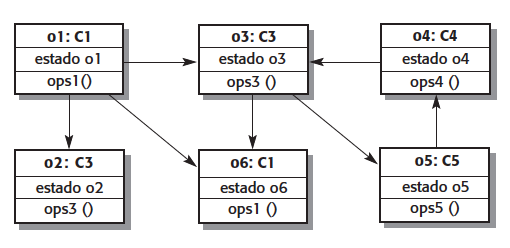
\includegraphics[scale=0.6]{imagens/figura-01.png}
  \caption{Um sistema constituído de objetos que interagem entre si.}
  \legend{Fonte: \cite{sommerville2003engenharia}}
  \label{fig:figura-01}
\end{figure}

Como afirma \citeonline{sommerville2003engenharia}, projeto orientado a objetos é parte do desenvolvimento orientado a objetos, em que uma estratégia orientada a objetos é utilizada em todo o processo de desenvolvimento:

\begin{itemize}
  \item A \textbf{análise orientada a objetos} se dedica a desenvolver um modelo orientado a objetos do domínio de aplicação. Os objetos identificados refletem entidades e operações que estão associadas com o problema a ser resolvido.

  \item O \textbf{projeto orientado a objetos} se dedica a desenvolver um modelo orientado a objetos de um sistema de software para implementar os requisitos identificados. Os objetos em um projeto orientado a objetos estão relacionados à solução do problema que está sendo resolvido. É possível que haj relacionamentos próximos entre alguns objetos do problema e alguns objetos da solução, mas o projetista, inevitavelmente, precisa adicionar novos objetos e transformar objetos do problema, a fim de implementar a solução.

  \item A \textbf{programação orientada a objetos} se ocupa de realizar um projeto de software utilizando uma linguagem de programação orientada a objetos, por exemplo, a linguagem Java, que aceita a implementação direta de objetos e fornece recursos para definir as classes de objetos.
\end{itemize}

A transição entre esses estágios de desenvolvimento deve ser contínua e direta,
com a mesma notação utilizada em cada um. Mover para o próximo envolve aprimorar o anterior, adicionando detalhes às classes existentes de objetos e inventando novas a fim de oferecer funcionalidades adicionais.

\section{Classes e objeto}

Para \cite{sommerville2003engenharia} ``objeto'' e ``orientado a objetos'' são
amplamente utilizados e aplicados a diferentes tipos de entidades, métodos de
projeto, sistemas e linguagens de programação. Contudo, existe uma aceitação
geral de que um objeto é um encapsulamento de informações, e isso se reflete na
definição de um objeto e de uma classe de objeto a seguir:

\begin{itemize}
  \item Um objeto é uma entidade que possui um estado e um conjunto definido de
  operações que operam nesse estado. O estado é representado por um conjunto de
  atributos de objeto. As operações associadas com o objeto fornecem serviços para outros objetos (clientes), que requisitam esses serviços quando alguma computação é necessária.

  \item Os objetos são criados de acordo com uma definição de classe de objetos 
  que serve como um template para criar objetos. Essa classe apresenta 
  declarações de todos os atributos e operações que devem ser associados a um 
  objeto dessa classe.
\end{itemize}

Em outras palavras, podemos dizer que classe é uma descrição generalizada que
descreve uma coleção de objetos similares, o qual, segundo 
\citeonline{pressman2016engenharia}, é um conceito orientado a objeto que 
encapsula dados e abstrações procedurais necessárias para descrever o conteúdo 
e comportamento de alguma entidade do mundo real.

Exemplos de objetos são: os \textbf{objetos físicos} (um livro, uma caneta), \textbf{funções de pessoas} para os sistemas (funcionário, cliente), eventos (uma compra, um  telefonema), \textbf{interações} entre outros objetos (um item de uma nota fiscal é uma interação entre uma compra e um produto do estoque) e \textbf{lugares} (loja matriz, revenda nordeste).

Para fins de estudo, e com objetivo mais didático, usaremos um cachorro como 
nosso ``objeto'':

\begin{figure}[H]
  \centering
  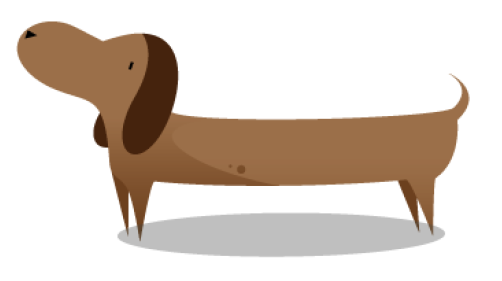
\includegraphics[scale=0.4]{imagens/cachorro-objeto.png}
  \caption{Representação de um objeto}
  \label{fig:cachorro-objeto}
\end{figure}

Ao analisar o objeto, deduz-se que há características pertencentes somente a 
ele. Tais como:

\begin{itemize}
  \item Nome;
  \item Idade;
  \item Comprimento de pelos;
  \item Cor dos pelos;
  \item Cor dos olhos;
  \item Peso, entre outros;
\end{itemize}

Tais características que descrevem um objeto são chamadas na orientação a 
objeto de atributos.

%\section{Instância}
%
%Uma instância de uma classe é um novo objeto criado dessa classe, com o operador \textbf{new}. Instanciar uma classe é criar um novo objeto do mesmo tipo dessa classe. Uma classe somente poderá ser utilizada após ser instanciada.

\section{Atributos}

Os objetos do mundo real tem propriedades que por sua vez possuem valores. 
Estes valores determinam o estado do objeto. Assim, na orientação a objeto, 
essas propriedades são chamadas de atributos. Logo, podemos dizer que esses atributos são semelhantes a variáveis ou campos que guardam os variados valores que os objetos podem receber como características.

\textbf{O estado de um objeto é um grupo de valores que estão em seus atributos em um certo momento}. \\

\begin{minipage}{\textwidth}
  \begin{minipage}[b]{0.49\textwidth}
    \centering
    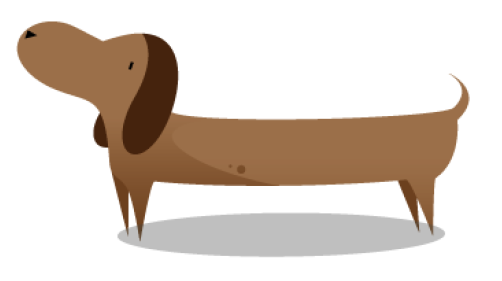
\includegraphics[scale=0.4]{imagens/cachorro-objeto.png}
    \captionof{figure}{Representação de um objeto}
    \label{fig:cachorro-objeto-1}
  \end{minipage}
  \hfill
  \begin{minipage}[b]{0.52\textwidth}
    \centering
    \begin{tabular}{|l|l|}
      \hline
      \multicolumn{2}{|c|}{Cachorro}      \\ \hline
        Nome:                 & Hubert    \\ \hline
        Idade:                & 2 anos    \\ \hline
        Tipo Pelo:            & Curtos    \\ \hline
        Cor dos pelos:        & Marrom    \\ \hline
        Cor dos olhos:        & Castanhos \\ \hline
        Peso                  & 5kg       \\ \hline
      \end{tabular}
      \captionof{table}{Atributos e valores}
    \end{minipage}
  \end{minipage} \\

  Outro objeto cachorro teria valores diferentes para estes mesmos atributos, como exemplo disto temos:

  \begin{minipage}{\textwidth}
    \begin{minipage}[b]{0.49\textwidth}
      \centering
      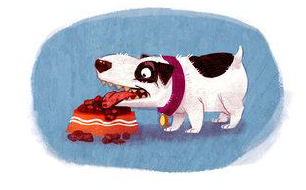
\includegraphics[scale=0.6]{imagens/cachorro-objeto-2.png}
      \captionof{figure}{Representação de um objeto}
      \label{fig:cachorro-objeto-2}
    \end{minipage}
    \hfill
    \begin{minipage}[b]{0.49\textwidth}
      \centering
      \begin{tabular}{|l|l|}
        \hline
        \multicolumn{2}{|c|}{Cachorro}      \\ \hline
          Nome:                 & Floks     \\ \hline
          Idade:                & 4 anos    \\ \hline
          Tipo pelo:            & Curtos    \\ \hline
          Cor dos pelos:        & Branco    \\ \hline
          Cor dos olhos:        & Castanhos \\ \hline
          Peso                  & 5kg       \\ \hline
        \end{tabular}
        \captionof{table}{Atributos e valores}
      \end{minipage}
    \end{minipage} \\ 

Para que os atributos de um objeto mudem de valor isso deve ser feito  exclusivamente por estímulos externos ou internos. Assim, a única maneira  de alterar os atributos dos objetos é disparando eventos que geram a mudança desses estados no objeto.

\section{Métodos}

São procedimentos ou funções que executam as ações específicas do objeto. 
Dessa forma, os métodos são as ações que o objeto é capaz de realizar. É 
através dos métodos que o objetos faz tudo, inclusive se manifesta e 
interage com outros objetos.

Um objetos expõe algum comportamento (ou seja, executa uma operação) ao 
receber um estímulo de outro objeto. É através de mensagens que um objeto 
requisita uma ação a outro objeto. Sendo esta mensagem uma solicitação a um 
objeto para que sejam executadas as rotinas a qual são nomeadas de Método da 
classe. Então os métodos assumem a responsabilidade de acessar ou alterar os 
atributos de um objeto.

Anteriormente no estudo do objeto cachorro foi enumerado uma série de métodos 
(ações), tais como: latir, babar, comer, sentar, etc.

\section{Herança}

O conceito de herança é um dos conceitos fundamentais de POO. Herança, na prática, significa a possibilidade de construir objetos especializados que herdam as características de objetos mais generalistas, ou ainda, a herança uma maneira de reutilizar código a medida que podemos aproveitar os atributos e métodos de classes já existentes para gerar novas classes mais específicas que aproveitarão os recursos da classe hierarquicamente superior \cite{evandroeduardoseronruiz2008}.

O conceito de herança mimetiza as características hierárquicas de vários sistemas reais, como por exemplo, os sistemas de classificação em biologia que, pode determinar como uma hierarquia o seguinte:

\begin{itemize}
    \item animais;
    \item vertebrados e invertebrados;
    \item mamíferos e aves;
    \item entre outras características mais específicas
\end{itemize}

\begin{figure}[H]
  \centering
  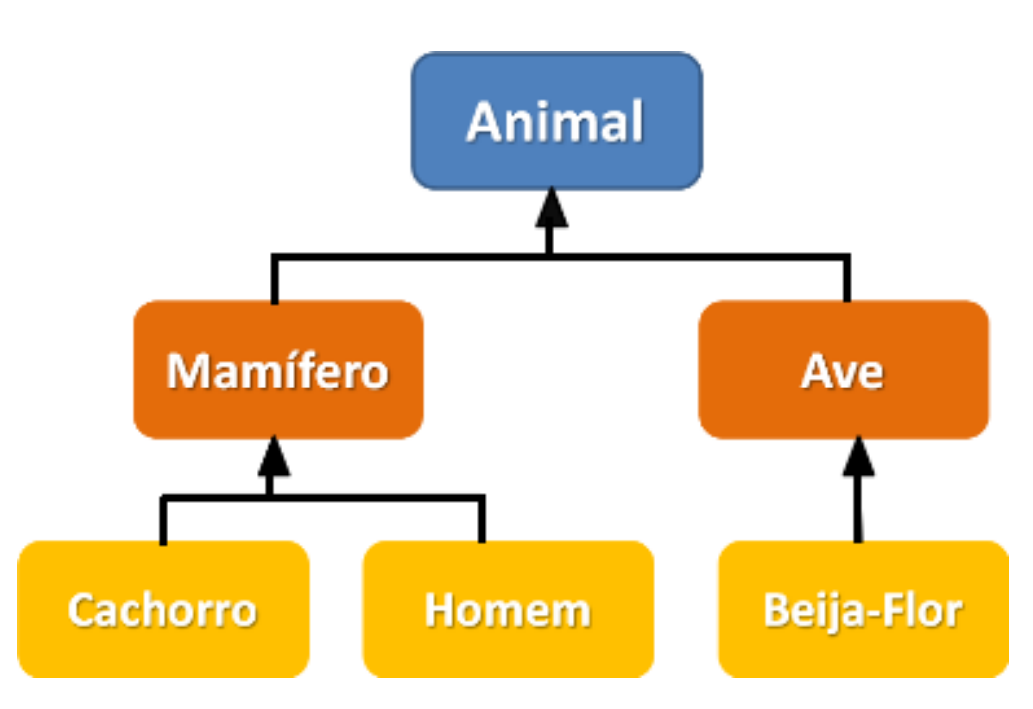
\includegraphics[scale=0.3]{imagens/heranca.png}
  \caption{Diagrama representando a herança entre as classes}
  \label{fig:heranca}
\end{figure}

\section{Classes abstratas}

Podemos dizer que as classes abstratas servem como modelo para outras classes que dela herdem (veremos herança nas próximas sessões), não podendo ser instanciada por si só. Para ter um objeto de uma classe abstrata é necessário criar uma classe mais especializada herdando dela e então instanciar essa nova classe. Os métodos da classe abstrata devem então serem sobrescritos nas classes filhas.


\subsection{Superclasses e subclasses}

Em POO todo objeto de uma classe construída pelo usuário da linguagem é também um objeto de outra classe.Por exemplo, na hierarquia da área da saúde, podemos dizer que pessoa é uma superclasse e que empregados é uma subclasse de pessoa.

Outra nomenclatura que é utilizada para especificar superclasses ou subclasses é a Generalização ou Especialização. No exemplo acima, pessoa é a generalização de empregado, e empregado é a especialização de pessoa conforme representado na Figura \ref{fig:sub-e-sup-classes}

Uma máxima que podemos guardar é: 

\begin{center}
\textbf{\textit{Uma subclasse guarda a relação é um com a superclasse.}}    
\end{center}

\begin{figure}[H]
  \centering
  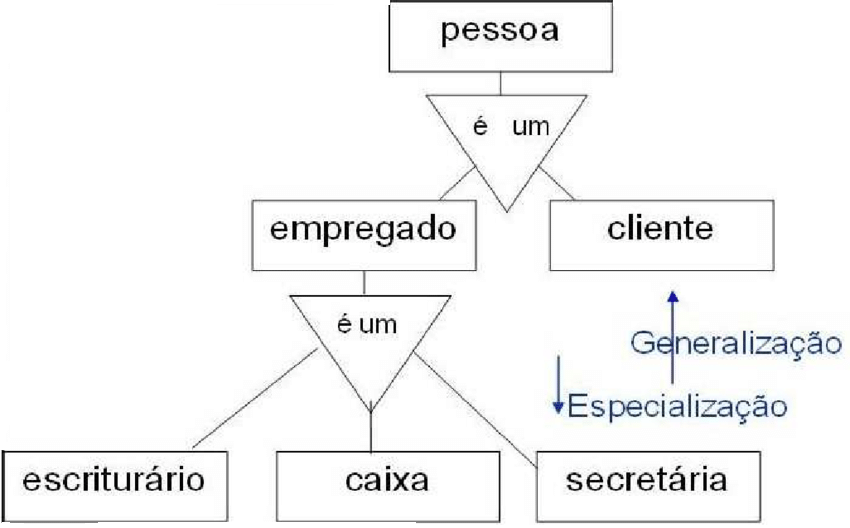
\includegraphics[scale=0.5]{imagens/sub-e-sup-classes.png}
  \caption{Superclassses e Subclasses}
  \legend{Fonte: \cite{articlelucas2009}}
  \label{fig:sub-e-sup-classes}
\end{figure}

\section{Exercícios de fixação}\label{exer:001}

\begin{enumerate}
    \item Para satisfazer as necessidades de informatização de uma biblioteca 
universitária um sistemas foi proposto para satisfazer algumas características:

\begin{itemize}
  \item Cadastro dos usuários da biblioteca com endereço completo. 
  Usuário são classificados em três grupos: professores, alunos e funcionário.  
  \item Cadastro das obras da biblioteca são classificados em: livros científicos, periódicos científicos, periódicos informativos, periódicos diversos, entretenimento, etc.
  \item Linguagem usada no exemplar da obra.
  \item Mídia que armazena o exemplar da obra.
  \item Autores da obra com o controle da nacionalidade dos mesmos.
  \item Editoras dos exemplares com ano de edição referente a cada exemplar.
\end{itemize}

Identifique os possíveis objetos com seus atributos e métodos respectivos.

\item \textbf{Desafio:} Pesquise sobre os pontos negativos da orientação a objeto, principalmente sobre os conceitos de Coesão e Acoplamento.
\end{enumerate}

\section{Mensagem}

Mensagens são requisições enviadas de um objeto para outro, para que o objeto ``receptor'' forneça algum resultado desejado por meio da execução de uma operação. As trocas de mensagem funcionam como uma fábrica que
recebe uma ordem de produção (mensagem de solicitação), processa essa ordem (operações) utilizando matéria-prima (atributos) e gera um produto final (mensagem de resposta).

\begin{figure}[H]
  \centering
  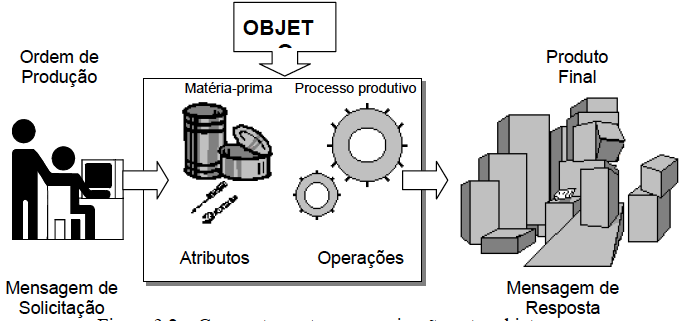
\includegraphics[scale=0.5]{imagens/analogia-mensagens.png}
  \caption{Comportamento e comunicação entre objetos}
  \label{}
\end{figure}

\section{Encapsulamento}

Cada objeto é visto como o encapsulamento do seu estado interno, suas mensagens e seus métodos. A estrutura do estado e dos pares "mensagem - método" são todas definidas através da classe à qual o objeto pertence.

\begin{itemize}
  \item A encapsulação de dados com o código que os manipula em classes é a principal vantagem da Orientação a Objeto
  \item No sentido de não quebrar a encapsulação, é muito importante que os membros de uma classe (atributos e métodos) sejam visíveis apenas onde estritamente necessário (A lei é: "Não posso quebrar o que não posso acessar").
\end{itemize}

\subsection{Especificadores de controle de acesso}

Juntamente com a ideia de encapsulamento nós também possuimos os especificadores de controle de acesso ou visibilidades. A visibilidade é a maneira com a qual o desenvolvedor proibe ou permite acesso a determinados métodos ou atributos de uma classe, como pode ser visto na Figura \ref{fig:encapsulamento}. Neste sentido, o objeto formado possuirá as mesmas definições declaradas pela classe.

\subsubsection{A visibilidade public}
\begin{itemize}
  \item Quem tem acesso à classe tem acesso também a qualquer membro com visibilidade public;
  \item O alvo aqui é o programador cliente que usa suas classes;
  \item É raro ter atributos públicos mas é comum ter métodos públicos.
\end{itemize}

\subsubsection{A visibilidade private}
\begin{itemize}
  \item O membro private não é acessível fora da classe;
  \item A intenção aqui é permitir que apenas você que escreve a classe possa usar esse membro.
\end{itemize}

\subsubsection{A visibilidade protected}
\begin{itemize}
  \item O membro protected é acessível à classe e a suas subclasses;
  \item A intenção é dar acesso ao programadores que estenderão sua classe.
\end{itemize}

\begin{figure}[H]
  \centering
  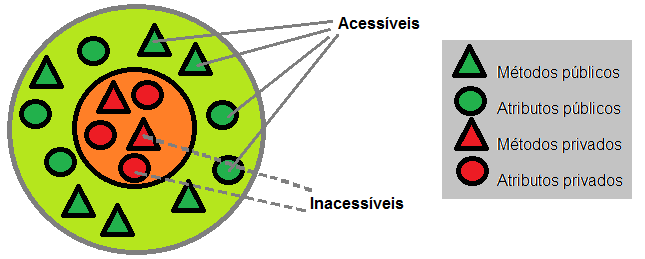
\includegraphics[scale=0.5]{imagens/encapsulamento.png}
  \caption{Encapsulamento}
  \label{fig:encapsulamento}
\end{figure}

\section{Polimorfismo}

É a propriedade que permite que a mesma mensagem seja enviada a diferentes objetos e que cada objeto execute a operação que é apropriada à sua classe. No caso de polimorfismo, é necessário que os métodos tenham exatamente a mesma identificação, sendo utilizado o mecanismo de redefinição de métodos.

No exemplo utilizado na Figura \ref{fig:polimorfismo}, podemos perceber que diferentes objetos, quando é solicitado a mesmo ação, se comportam de maneira diferente. Similiar a objetos do mundo real, na Orientação a Objetos, o comportamento por meio do polimorfismo acontece da mesma forma. 

\begin{figure}[H]
  \centering
  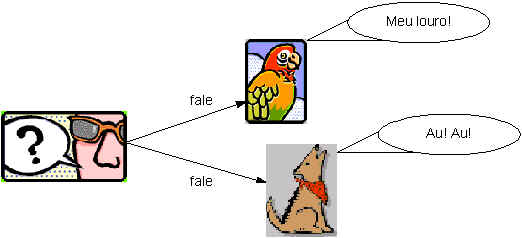
\includegraphics[scale=0.2]{imagens/polianimais.jpg}
  \caption{Polimorfismo}
  \label{fig:polimorfismo}
\end{figure}

\section{Conceitos estudados até este momento}

Para ilustrar, a tabela abaixo contém um resumo e um exemplo de todos estes conceitos.

\begin{table}[H]
  \resizebox{\textwidth}{!}{%
  \begin{tabular}{|l|l|l|}
  \hline
  \multicolumn{1}{|c|}{\textbf{Palavra-Chave}} & \multicolumn{1}{c|}{\textbf{Breve Definição}} & \multicolumn{1}{c|}{\textbf{Exemplo}} \\ \hline
  Classe & \begin{tabular}[c]{@{}l@{}}Agrupamento de objetos similares que\\ apresentam os mesmos atributos e operações\end{tabular} & Indivíduo, caracterizando as pessoas do mundo \\ \hline
  Atributo & \begin{tabular}[c]{@{}l@{}}Característica particular de uma ocorrência da\\ classe\end{tabular} & \begin{tabular}[c]{@{}l@{}}Indivíduo possui nome, sexo, data de\\ nascimento\end{tabular} \\ \hline
  Operações & \begin{tabular}[c]{@{}l@{}}Lógica contida em uma classe para designar-lhe\\ um comportamento\end{tabular} & \begin{tabular}[c]{@{}l@{}}Cálculo da idade de uma pessoa em uma classe\\ (Indivíduo)\end{tabular} \\ \hline
  Encapsulamento & \begin{tabular}[c]{@{}l@{}}Combinação de atributos e operações de uma\\ classe\end{tabular} & \begin{tabular}[c]{@{}l@{}}Atributo: data de nascimento\\ Operação: cálculo da idade\end{tabular} \\ \hline
  Herança & \begin{tabular}[c]{@{}l@{}}Compartilhamento pela subclasse dos atributos\\ e operações da classe pai\end{tabular} & \begin{tabular}[c]{@{}l@{}}Subclasse (Eucalipto) compartilha atributos e\\ operações da classe (Árvore)\end{tabular} \\ \hline
  Subclasse & Característica particular de uma classe & \begin{tabular}[c]{@{}l@{}}Classe (Árvore),Subclasses (Ipê, Eucalipto,\\ Jacarandá, etc.)\end{tabular} \\ \hline
  Instância de Classe & \begin{tabular}[c]{@{}l@{}}Uma ocorrência específica de uma classe. É o\\ mesmo que objeto\end{tabular} & \begin{tabular}[c]{@{}l@{}}Uma pessoa, uma organização ou um\\ equipamento\end{tabular} \\ \hline
  Objeto & \begin{tabular}[c]{@{}l@{}}Elemento do mundo real (natureza). Sinônimo\\ de instância de classe\end{tabular} & \begin{tabular}[c]{@{}l@{}}Pessoa “Fulano de Tal”, Organização “ACM”,\\ Equipamento “Extintor”\end{tabular} \\ \hline
  Mensagem & \begin{tabular}[c]{@{}l@{}}Uma solicitação entre objetos para invocar certa\\ operação\end{tabular} & Informar idade da pessoa “Fulano de Tal” \\ \hline
  Polimorfismo & \begin{tabular}[c]{@{}l@{}}Habilidade para usar a mesma mensagem para\\ invocar comportamentos diferentes do objeto\end{tabular} & \begin{tabular}[c]{@{}l@{}}Chamada da operação: “Calcular Saldo” de\\ correntista. Invoca as derivações\\ correspondentes para cálculo de saldo de\\ poupança, renda fixa, etc.\end{tabular} \\ \hline
  \end{tabular}%
  }
  \end{table}

  \section{Exercícios de fixação}

  Baseando-se nas explicações em aula e em suas anotações, responda as seguintes questões:

  \begin{enumerate}
    \item O que é a Programação Orientada a Objetos e qual a sua relação com o Projeto orientado e objeto. Aponte as diferenças e similitudes em ambos os conceitos.
    \item   Um ponto importante que deve ser claro para que possamos atingir o objetivo de nossa disciplina é o conceito sobre classes e objetos. Explique o que são e de exemplos do seu cotidiano para reforçar a ideia.
    \item O que são atributos e métodos? Defina cada um e de exemplos para afirmar sua resposta. Obs: Caso possível, use o exemplo anterior.
    \item Um dos pilares da orientação a objeto é a Herança. Desenho um gráfico, semelhante ao da Figura \ref{fig:heranca}, representado a sua Árvore Genealógica. Caso consiga, vá té seus bisavós. 
    \item Utilizando o exercício anterior. Represente, por meio de setas, as possíveis trocas de mensagem entre os objetos que você pode identificar. 
  \end{enumerate}
  



  

  



